
%(BEGIN_QUESTION)
% Copyright 2006, Tony R. Kuphaldt, released under the Creative Commons Attribution License (v 1.0)
% This means you may do almost anything with this work of mine, so long as you give me proper credit

I prosesser med spesielt farlige medier brukes ofte ``double block-and-bleed''-manifolder for å isolere instrumenter fra prosessrør.  Se dette eksemplet:

$$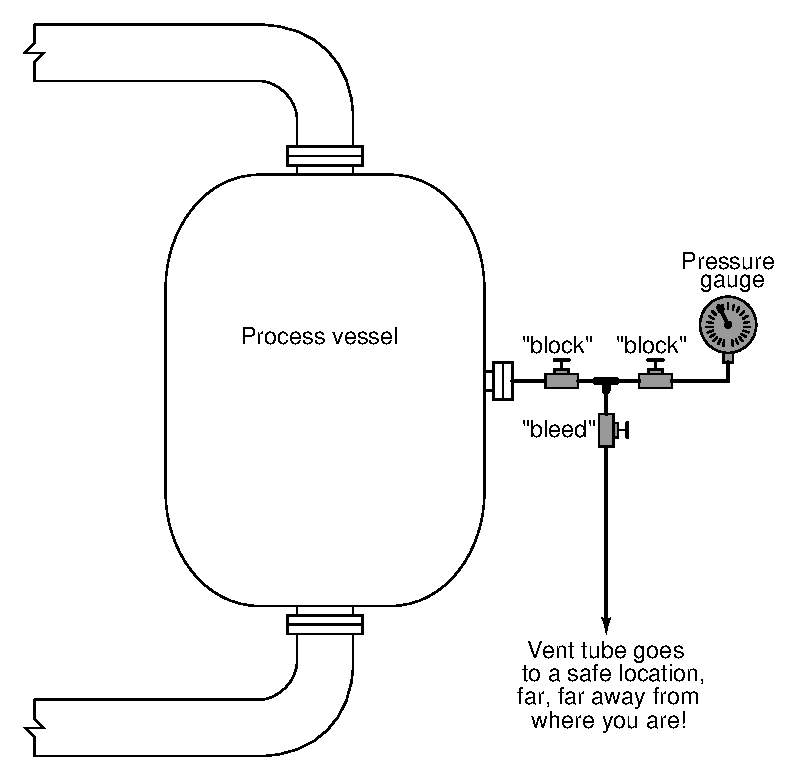
\includegraphics[width=15.5cm]{i00210x01.eps}$$

Beskriv riktig prosedyre for åpning/lukking av block- og bleed-ventiler ved uttak og remontering av instrument gjennom en slik manifold.

\underbar{file i00210}
%(END_QUESTION)





%(BEGIN_ANSWER)

Ta manometeret ut av drift:

\begin{itemize}
\item{} Lukk ``block''-ventilen nærmest prosessen.
\item{} Åpne ``bleed''-ventilen.  Overvåk trykkindikasjonen for å bekrefte at trykket går mot atmosfære.
\item{} Lukk ``block''-ventilen nærmest instrumentet.
\item{} Lukk ``bleed''-ventilen.
\item{} Sett lockout-merker på alle tre ventilhåndtak.
\item{} Demonter manometeret.
\end{itemize}

Hvis prosessmediet er spesielt farlig, kan instrumentet kreve de-kontaminering før det kobles til kalibreringsutstyr i verksted.

\vskip 10pt

Sette manometeret tilbake i drift:

\begin{itemize}
\item{} Fjern lockout-merker.
\item{} Åpne ``bleed''-ventilen (for å avlaste eventuelt oppbygget trykk mellom de to lukkede block-ventilene ved lekkasje i første block-ventil).
\item{} Monter manometeret.
\item{} Åpne ``block''-ventilen nærmest instrumentet.
\item{} Lukk ``bleed''-ventilen.
\item{} Åpne ``block''-ventilen nærmest prosessen.
\end{itemize}

%(END_ANSWER)





%(BEGIN_NOTES)

Eksempler på prosesser der double block/bleed kan være nødvendig:

\begin{itemize}
\goodbreak
\item{} Svært brennbare væsker eller gasser
\item{} Svært giftige væsker eller gasser
\item{} Høytrykks væsker eller gasser
\item{} Kombinasjoner av disse
\end{itemize}

%INDEX% Safety, isolation valves: double block and bleed

%(END_NOTES)

